\documentclass{ctexart}
\usepackage{PhysicalChemistryNote}

\begin{document}\pagestyle{plain}
\noindent\tbf{\LARGE 7C 反应机理与速率方程的推导}\vspace{15pt}\\
\indent 化学反应在大多数情况下并不是一蹴而就的.例如葡萄糖\ce{C6H12O6}在你的身体里被氧化的过程:%
\ce{C6H12O6 + 6O2 -> 6CO2 + 6H2O}.显然,让一个\ce{C6H12O6}分子与六个\ce{O2}分子一步到位地生成%
六个\ce{CO2}分子与六个\ce{6H2O}分子是不大现实的,这需要所有\ce{O2}同时以合适的角度接近并发生反应,%
这一概率是非常低的.事实上我们知道,这一反应,乃至绝大多数反应都是通过数个步骤进行的,%
这些步骤构成了我们所讲的反应机理,并且也密切影响着反应的速率.\vspace{12pt}\\
\Section{7C.1 基元反应}
\Part{基元反应}
\indent 在前言中,我们说大部分反应都是通过数个步骤进行的.这些简单而基本的步骤就是我们所说的\tbf{基元反应}.
\begin{definition}[7C.1.1 基元反应]
    \tbf{基元反应}(或称\tbf{基本反应}),顾名思义,即最简单的化学反应步骤,是一个或多个化学物种直接作用,一步(即通过单一过渡态)转化为反应产物的过程.
\end{definition}
下面是几个常见的基元反应:
\begin{tightcenter}
    \ce{H. + Br2 -> HBr + Br.}\\
    \ce{CH3I + Cl- -> CH3Cl + I-}\\
    \ce{I2 -> 2I.}
\end{tightcenter}
可以看到,参与基元反应的物质并不一定是稳定的化合物,也可能是自由基等不稳定物种.并且,参与反应的分子数各不相同.
\begin{theorem}[7C.1.2 基元反应的分子数]
    基元反应的\tbf{分子数}是指参与基元反应的分子数.\\
    在\tbf{单分子反应}中,单个分子振动分解或发生重排.\\
    在\tbf{双分子反应}中,参与反应的两个分子以合适的方式碰撞,发生能量交换,键的生成和断裂等过程.\\
    一般而言,三分子反应已经很少见,而分子数大于等于四的基元反应几乎不存在.
\end{theorem}
基元反应,正由于其简单的特征,速率方程也十分简洁.
\begin{theorem}[7C.1.3 基元反应的速率方程]
    单分子基元反应对反应物为一级,其速率(以\ce{A -> P}为例)为$v=k\con{A}$.\\
    双分子基元反应对每个反应物都为一级(如果反应物相同就为二级),其速率(以\ce{A + B -> P}为例)为$v=k\con{A}\con{B}$,%
    或(以\ce{2A -> P}为例)为$v=k\con{A}^2$.
\end{theorem}
我们可以对上面的结论做定性的解释.%
在一定温度下,具有适合的能量的分子在总体中占的比例是一定的.因此,参与基元反应的物质的浓度越高,%
具有适合的能量的分子的浓度就越高,反应速率也就越快,并且对每个参与反应的分子的浓度都应当%
成正比例关系.\vspace{4pt}\\
\Part{微观可逆性原理和精细平衡原理}
\indent 直觉地来看,如果将描述物质运动的方程中的时间$t$和速度$v$替换成其负值,并不影响运动方程%
的成立.因此,运动的过程是可以通过恰好相反的方向进行的,而它们遵守相同的物理规律.这就是力学中的\tbf{时间反演对称性}%
\footnote{说得粗糙一些,这和时间倒流在某种程度上是一致的.如果你看过Christopher Nolan执导的电影《信条》,可能对这样的现象会有更为直观的认识.}.
\begin{hint}
    这一“直觉”事实上在经典力学和量子力学中都可以被证明,但由于涉及到一些复杂的物理知识,故在此并不给出.\\
    需要注意的是,由于我们在这里讨论的仅仅是单个或少数几个物体(即分子),因此尚不具有统计意义.%
    这要与热力学第二定律做区分.\\
    你可以简单地认为,力学肯定的是微观过程的可逆性,而统计物理学(以及热力学)肯定的是宏观过程的不可逆性,%
    两者讨论的范畴并不相同,因此也没有矛盾之处.
\end{hint}
以上我们从力学的角度讨论了时间反演对称性.它告诉我们,化学过程中反应的微粒服从力学方程(如基元反应中反应物微粒单次碰撞行为),%
则在正,逆反应过程中所经历的途径是相同的,逆过程要经历正过程的所有状态,就像一部电影从后往前倒过来放映,%
片中的一切动作是正常放映时动作的完全逆转;同时,在沿着反应坐标移动形成并最后解体的活化络合物的组成和结构在两个方向上是相同的,只不过动量的符号相反.%
由此,我们可以提出时间反演对称在化学动力学中的表述.
\begin{theorem}[7C.1.4 微观可逆性原理]
    如果一个正反应是基元反应,那么它的逆反应也是基元反应,且正逆反应具有相同的活化络合物(即中间体).
\end{theorem}
微观可逆性原理对假设反应厉程有明显的制约:它要求设想的反应机理中任一基元反应的逆反应不应是不可能的反应.%
如四乙基铅的气相分解反应:\ce{Pb(C2H5)4 -> Pb + 4C2H5.},逆反应是不可能发生的五分子反应,所以该反应不可能是基元反应.\\
\indent 到目前为止,我们似乎仍未考虑反应达到平衡的情形.此时,总体正反应和逆反应的速率相等,%
各物质的浓度不再随时间变化.那么具体到每个基元反应上又是何种情况呢?%
为此,人们提出了精细平衡原理.
\begin{theorem}[7C.1.5 精细平衡原理]
    平衡时,宏观体系中每一个基元反应的速率一定等于其逆反应的速率.
\end{theorem}
在化学动力学的范畴中,这也是一条可以被证明的定理.因此,这从根本上否定了平衡时存在单向不可逆循环的存在.%
每个基元反应必然存在其逆反应,且平衡时正逆反应的速率相等.%
我们将在之后看到精细平衡原理对反应机理的限制.\\
\indent 最后,需要说明的是尽管基元反应都存在逆反应,但很多基元反应的逆反应的速率非常缓慢,以至于可以忽略不计,%
因此我们近似地认为这些反应是不可逆的.这与我们在\tbf{5B.3.5}中说到的一致,即在动力学中,可逆是绝对的,不可逆是相对的.\vspace{12pt}\\
\Section{7C.2 连续反应动力学}
\Part{两步连续反应的积分速率方程}
\indent 基元反应最简单的组合方式就是连续地发生,通过几个连续的步骤完成反应.例如\ce{^{239}U}衰变为%
\ce{^{239}Pu},就是通过下面的连续$\beta$衰变进行的:
\begin{tightcenter}
    \ce{^{239}U ->T[$t_{1/2}=23.5$ min] ^{239}Np ->T[$t_{1/2}=2.35$ d] ^{239}Pu}
\end{tightcenter}
现在,我们尝试用数学方法推导最简单的连续反应——两步连续反应的积分速率方程.
\begin{derivation}
    考虑连续反应
    \begin{tightcenter}
        \ce{A ->T[$k_1$] I ->T[$k_2$] P}
    \end{tightcenter}
    对于\ce{A}而言,它的消耗是一个一级反应,满足
    \[\con{A}=\con{A}_0\e^{-k_1t}\]
    而\ce{I}满足
    \[\dfrac{\di\con{I}}{\di t}=k_1\con{A}-k_2\con{I}\]
    代入$\con{A}$的表达式即有
    \[\dfrac{\di\con{I}}{\di t}+k_2\con{I}=\con{A}_0\e^{-k_1t}\]
    这是一个一阶线性常微分方程.我们已经讲过它的解法,即常数变易法.该方程对应的齐次方程
    \[\dfrac{\di\con{I}}{\di t}+k_2\con{I}=0\]
    的通解为
    \[\con{I}=C\e^{-k_2t}\]
    令$\con{I}=C(t)\e^{-k_2t}$,代入原方程即有
    \[C'(t)\e^{-k_2t}=\con{A}_0\e^{-k_1t}\]
    于是
    \[C'(t)=\con{A}_0\e^{\left(k_2-k_1\right)t}\]
    如果$k_1\neq k_2$,那么积分可得
    \[C(t)=\dfrac{\con{A}_0}{k_2-k_1}\e^{\left(k_2-k_1\right)t}+I\]
    其中$I$为待定的积分常数.代回$\con{I}$的表达式就有
    \[\con{I}=\dfrac{\con{A}_0}{k_2-k_1}\e^{-k_1t}+I\e^{-k_2t}\]
    由于起始是并没有中间产物\ce{I}的产生,因此$t=0$时$\con{I}=0$.代入上式即可得积分常数,整理可得
    \[\con{I}=\dfrac{\con{A}_0}{k_2-k_1}\left(\e^{-k_1t}-\e^{-k_2t}\right)\]
    从而反应的速率(这里以生成\ce{P}的速率计)为
    \[v=\dfrac{\di\con{P}}{\di t}=k_2\con{I}=\dfrac{k_2\con{A}_0}{k_2-k_1}\left(\e^{-k_1t}-\e^{-k_2t}\right)\]
    由于$\con{A}+\con{I}+\con{P}=\con{A_0}$总是成立,于是
    \[\con{P}=\left(1+\dfrac{k_1\e^{-k_2t}-k_2\e^{-k_1t}}{k_2-k_1}\right)\con{A}_0\]
    这就是两步连续反应的速率方程.
\end{derivation}
\begin{theorem}[7C.2.1 两步连续反应的积分速率方程]
    连续反应\ce{A ->T[$k_1$] I ->T[$k_2$] P}的积分速率方程为
    \[\con{P}=\left(1+\dfrac{k_1\e^{-k_2t}-k_2\e^{-k_1t}}{k_2-k_1}\right)\con{A}_0\]

\end{theorem}
至于更多步的连续反应,虽然在理论上不过是多次应用常数变易法解微分方程,但其计算的复杂程度却是迅速增长的\footnote{但这似乎并不妨碍某些丧心病狂的出题人考察多步连续反应的积分速率方程.}.%
因此大多数情况下,我们也不要求连续反应的精确的积分速率方程,而是采取合理的近似以简化计算.\vspace{4pt}\\
\Part{稳态近似}
\indent 当反应机理变得更加复杂(例如存在逆反应或多步连续反应时),微分方程可能就没有显式的解,%
精确求解这样的体系也会使得计算难度大幅增加.因此我们需要想办法做一些合理的近似以简化计算.%
为此,我们先观察以下情况下两步连续反应的各物质浓度随时间变化的图像.
\begin{figure}[H]
    \centering\documentclass{standalone}
\usepackage{PhysicalChemistryNote}
\begin{document}
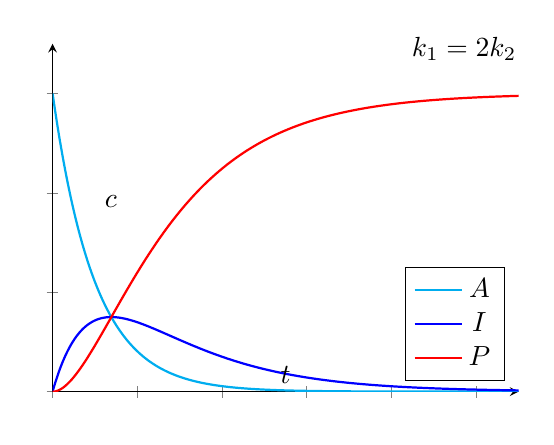
\begin{tikzpicture}
    \begin{axis}[
        title = {$k_1=2k_2$},
        title style={at={(0.75,1)},anchor=north west},
        width = 7.5cm,
        height = 6cm,
        legend pos = south east,
        x label style={at={(axis description cs:0.5,0.1)},anchor=north},
        y label style={at={(axis description cs:0.125,0.5)},rotate=270,anchor=south},
        xlabel = {$t$},
        ylabel = {$c$},
        axis lines = left,
        ymax = 3.5,
        domain = 0:5.5,
        samples = 400,
        xticklabels={},
        yticklabels={}
    ]
    \addplot [thick, cyan] {3*e^(-2*x)};
    \addplot [thick, blue] {3*(e^(-x)-e^(-2*x))};
    \addplot [thick, red] {3*(1-(2*e^(-x)-e^(-2*x)))};
    \legend {$\con{A}$,$\con{I}$,$\con{P}$}
    \end{axis}
\end{tikzpicture}
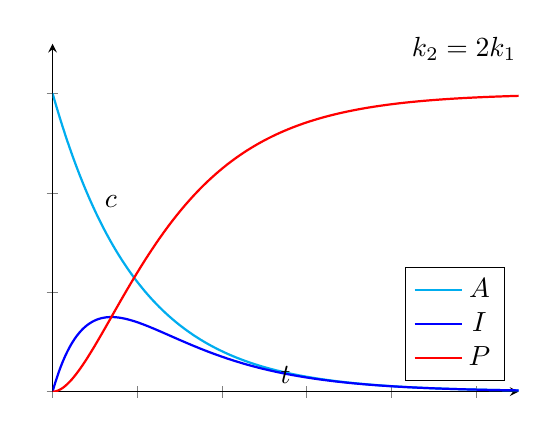
\begin{tikzpicture}
    \begin{axis}[
        title = {$k_2=2k_1$},
        title style={at={(0.75,1)},anchor=north west},
        width = 7.5cm,
        height = 6cm,
        legend pos = south east,
        x label style={at={(axis description cs:0.5,0.1)},anchor=north},
        y label style={at={(axis description cs:0.125,0.5)},rotate=270,anchor=south},
        xlabel = {$t$},
        ylabel = {$c$},
        axis lines = left,
        ymax = 3.5,
        domain = 0:5.5,
        samples = 400,
        xticklabels={},
        yticklabels={}
    ]
    \addplot [thick, cyan] {3*e^(-x)};
    \addplot [thick, blue] {3*(e^(-x)-e^(-2*x))};
    \addplot [thick, red] {3*(1-(2*e^(-x)-e^(-2*x)))};
    \legend {$\con{A}$,$\con{I}$,$\con{P}$}
    \end{axis}
\end{tikzpicture}
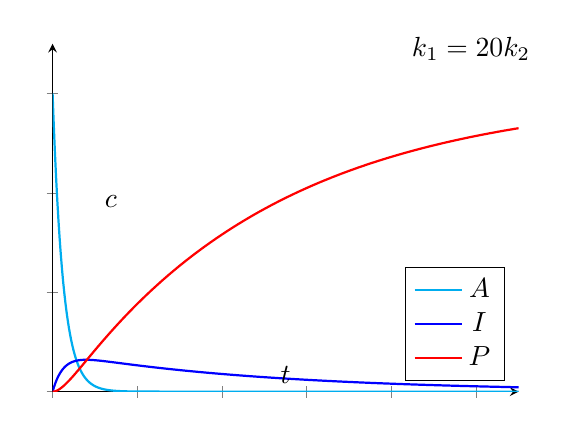
\begin{tikzpicture}
    \begin{axis}[
        title = {$k_1=20k_2$},
        title style={at={(0.75,1)},anchor=north west},
        width = 7.5cm,
        height = 6cm,
        legend pos = south east,
        x label style={at={(axis description cs:0.5,0.1)},anchor=north},
        y label style={at={(axis description cs:0.125,0.5)},rotate=270,anchor=south},
        xlabel = {$t$},
        ylabel = {$c$},
        axis lines = left,
        ymax = 3.5,
        domain = 0:5.5,
        samples = 400,
        xticklabels={},
        yticklabels={}
    ]
    \addplot [thick, cyan] {3*e^(-8*x)};
    \addplot [thick, blue] {3/7.6*(e^(-0.4*x)-e^(-8*x))};
    \addplot [thick, red] {3*(1+(0.4*e^(-8*x)-8*e^(-0.4*x))/7.6)};
    \legend {$\con{A}$,$\con{I}$,$\con{P}$}
    \end{axis}
\end{tikzpicture}
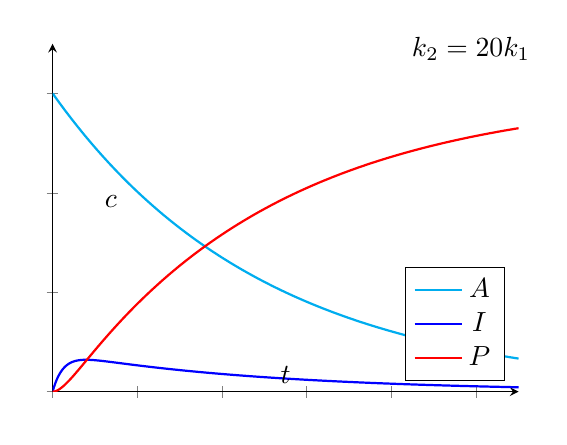
\begin{tikzpicture}
    \begin{axis}[
        title = {$k_2=20k_1$},
        title style={at={(0.75,1)},anchor=north west},
        width = 7.5cm,
        height = 6cm,
        legend pos = south east,
        x label style={at={(axis description cs:0.5,0.1)},anchor=north},
        y label style={at={(axis description cs:0.125,0.5)},rotate=270,anchor=south},
        xlabel = {$t$},
        ylabel = {$c$},
        axis lines = left,
        ymax = 3.5,
        domain = 0:5.5,
        samples = 400,
        xticklabels={},
        yticklabels={}
    ]
    \addplot [thick, cyan] {3*e^(-0.4*x)};
    \addplot [thick, blue] {3/7.6*(e^(-0.4*x)-e^(-8*x))};
    \addplot [thick, red] {3*(1+(0.4*e^(-8*x)-8*e^(-0.4*x))/7.6)};
    \legend {$\con{A}$,$\con{I}$,$\con{P}$}
    \end{axis}
\end{tikzpicture}
\end{document}
\end{figure}
当$k_1<k_2$时,
\end{document}